\section{Der Spannungszustand\label{spannung:section:Der Spannungsustand}}
\rhead{Der Spannungszustand}
Ein Spannungszustand ist durch alle Spannungen, welche in einem beliebigen Punkt im Körper wirken, definiert (siehe Abbildung~\ref{spannung:Bild2}).
Änderungen der äusseren Kräfte verändern die inneren Spannungszustände im Material.
Um alle Spannungen eines Punktes darstellen zu können, wird ein infinitesimales Bodenelement in Form eines Würfels modellhaft vorgestellt.
Man spricht auch von einem Elementarwürfel, da dieser elementar klein ist.

\begin{figure}
	\centering
	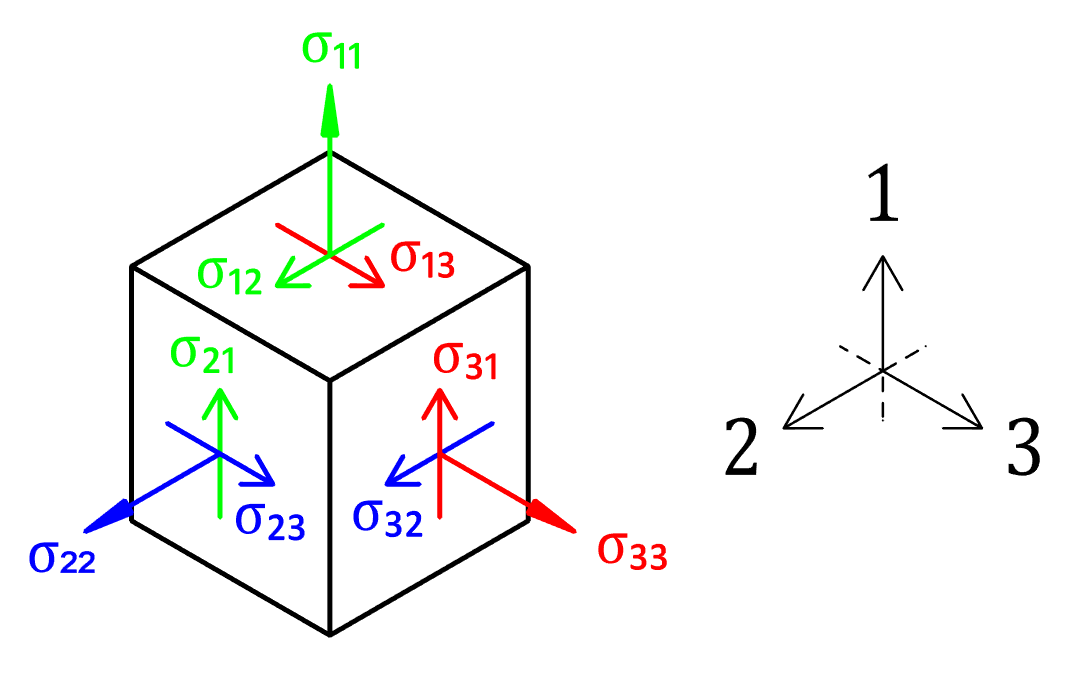
\includegraphics[width=0.4\linewidth,keepaspectratio]{papers/spannung/Grafiken/Bild2.png}
	\caption{Infinitesimales Bodenelement mit den 9 Spannungen}
	\label{fig:Bild2}
\end{figure}

Es werden jeweils drei Seiten dieses Würfels betrachtet, wobei die drei gegenüberliegenden Seiten im Betrag die selben Spannungen aufweisen,
sodass der Elementarwürfel im Gleichgewicht ist.
Wäre dieses Gleichgewicht nicht vorhanden, käme es zu Verschiebungen und Drehungen.
Das infinitesimale Bodenteilchen hat die Koordinaten $1$, $2$, $3$.
Veränderungen der Normalspannungen können durch Schubspannungen kompensiert werden und umgekehrt.
So sind insgesamt neun verschiedene Spannungen möglich, wobei drei Normal- und sechs Schubspannungen sind.
Normalspannungen wirken normal (mit rechtem Winkel) zur angreifenden Fläche und Schubspannungen parallel zur angreifenden Fläche.
Alle Beträge dieser neun Spannungen am Elementarwürfel bilden den Spannungszustand.
Daraus können die äquivalenten Dehnungen $\varepsilon$ mit Hilfe des Hook'schen Gesetz berechnet werden.
Daher gibt es auch den entsprechenden Dehnungszustand.


\section{Spannungszustand\label{spannung:section:Spannungsustand}}
\rhead{Spannungszustand}

Im einachsigen Spannungszustand herrscht nur die Normalspannung $\sigma_{11}$ (siehe Abbildung~\ref{spannung:Bild1}).
Das Hook'sche Gesetz beschreibt genau diesen 1D Spannungszustand.
Nach Hooke gilt:
\[
F
\sim
\Delta l
.
\]
Teilt man beide Seiten durch die Konstanten $A$ und $l_0$, erhält man
\[
\frac{F}{A}
=
\sigma
\sim
\varepsilon
=
\frac{\Delta l}{l_0}
\]
und somit
\[
\sigma
\sim
\varepsilon
,
\]
mit
\begin{align*}
	l_0 &= \text{Länge zu Beginn [\si{\meter}]} \\
	  A &= \text{Fläche [\si{\meter\squared}].}
\end{align*}
Diese Beziehung gilt bei linear-elastischen Materialien, welche reversible Verformungen zulassen.
Es ist praktisch die relative Dehnung $\varepsilon$ anzugeben und nicht eine absolute Längenänderung $\Delta l$.
\begin{figure}
	\centering
	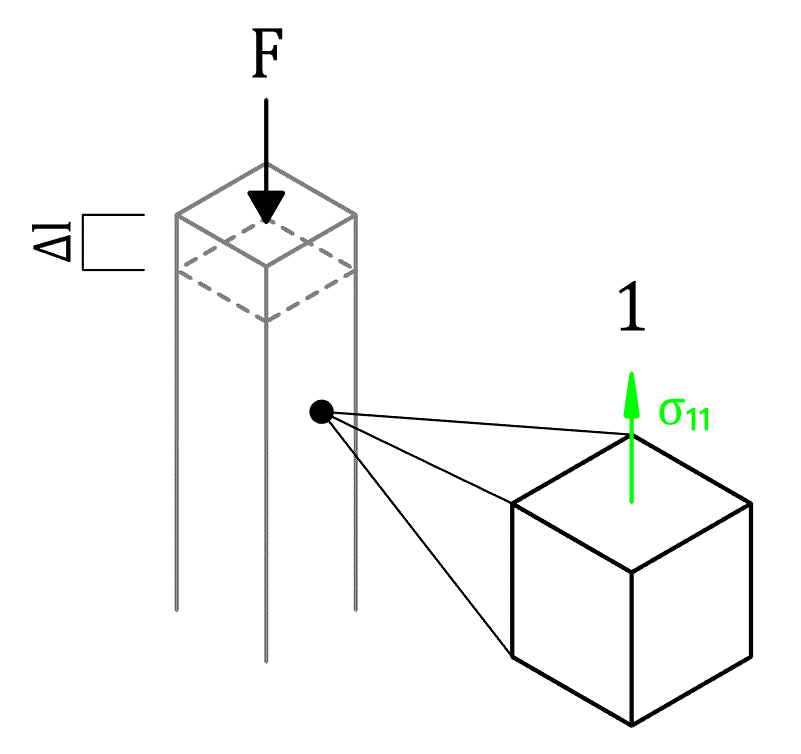
\includegraphics[width=0.35\linewidth,keepaspectratio]{papers/spannung/Grafiken/Bild1.png}
	\caption{1D Spannungszustand aus einer quaderförmigen Bodenprobe}
	\label{fig:Bild1}
\end{figure}
Mithilfe vom Elastizitätsmodul $E$ als Proportionalitätskonstante lässt sich der eindimensionale Fall mit
\[
\sigma
=
E\cdot\varepsilon
\]
beschreiben.
Im Falle, dass $E$ nicht konstant ist, kann dieser näherungsweise durch
\[
E
=
\frac{\Delta\sigma}{\Delta\varepsilon}
\]
ausgedrückt werden.